\documentclass[tikz]{standalone}
\usepackage{amsmath}
\usepackage{amssymb}
\usepackage{amsfonts}
\usepackage{tikz}

\thispagestyle{empty}
\begin{document}

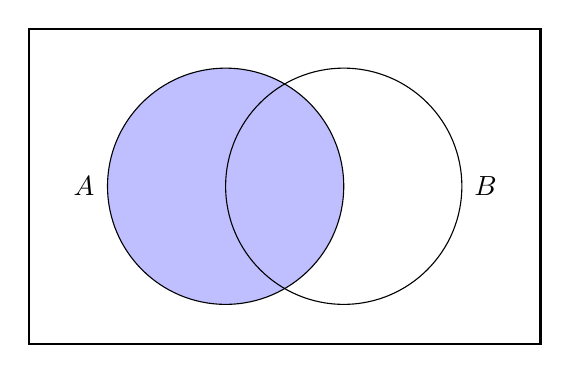
\begin{tikzpicture}
% Universal set rectangle
\draw[thick] (-2.5,-2) rectangle (4,2);

% Highlight A only
\begin{scope}
\clip (-2.5,-2) rectangle (4,2);          
\fill[blue!25] (0,0) circle (1.5cm);       % Fill A
\end{scope}

% Set A and B outlines
\draw (0,0) circle (1.5cm);
\draw (1.5,0) circle (1.5cm);
\node at (-1.8, 0) {$A$};
\node at (3.3, 0) {$B$};

\end{tikzpicture}
\end{document}
